\ctpartquote{}
\ctparttext{}
\part{Appendices}

\chapter{Supplementary information}
\label{ch:04-A:supdata}

    \section{Sparse convolution in Chromosight}
    \label{sec:04-A-01:convolution}

The explanation below describes how Chromosight reformulates convolution into a matrix multiplication problem to better handle large sparse matrices. The algorithm is inspired from \cite{NeuralNetwork2D}. For brevity, we call the operation "convolution" throughout the section, although cross-correlation could be considered more accurate as we do not transpose the kernel. Let S be the signal (Hi-C) matrix and K the kernel matrix.

\begin{equation}
    S = 
    \begin{bmatrix}
        4 & 2 & 1 \\
        2 & 4 & 1 \\
        1 & 1 & 3
    \end{bmatrix}
    K =
    \begin{bmatrix}
        10 & 12 \\
        11 & 13 \\
    \end{bmatrix}
\end{equation}

The dimensions of the desired convolution output are defined by:

\begin{equation}
    (m_S - m_K + 1) \times (n_S - n_K + 1)
\end{equation}

Note this corresponds to a convolution in "valid" mode, where edge values are truncated.

We transform each column of the kernel into a Toeplitz matrix with the same number of columns as the input signal. In this matriix, each value along the diagonals is constant.

\begin{align}
    T_0 &=
    \begin{bmatrix}
        10 & 11 & 0 \\
        0  & 10 & 11
    \end{bmatrix} &
    T_1 &=
    \begin{bmatrix}
        12 & 13 & 0 \\
        0  & 12 & 13
    \end{bmatrix}
\end{align}

The convolution of the signal and kernel can now be replaced by a sum of dot products between the signal and Toeplitz matrices built from the column filters. For each dot product, the signal is shifted according to the order of filters to respect operations performed during convolution.

\begin{align}
    C &= S * K \\
      &= S[:, 0: sn-kn+1] \cdot T_0 + S[:, 1:sn-kn+2] \cdot T_1
\end{align}

Where $\cdot$ is the matrix dot product operator and $*$ is the convolution operator.
The complete convolution algorithm used in chromosight is given as pseudocode in algorithm \ref{alg:04-B-01:convolution}.

\begin{algorithm}
\caption{Calculate $C = S * K$ using matrix products}
\label{alg:04-B-01:convolution}
\begin{algorithmic}
\REQUIRE S, $m_S \times n_S$ matrix
\REQUIRE K, $m_K \times n_K$ matrix
\ENSURE $m_S >= m_K, n_S >= n_K$
\STATE Let $\left\{T_0, ..., T_{n_K}\right\}$ be $m_K \times n_S$ matrices
\STATE $y \leftarrow 0$
\WHILE{$y \neq n_K$}
    \STATE $t \leftarrow 0$
    \WHILE{$t \neq n_S$}
        \STATE $T_y[t, :] \leftarrow K[:, t]^T$
    \ENDWHILE
\ENDWHILE
\STATE Let $C$ be a $(m_S - m_K + 1) \times (n_S - n_K + 1)$ matrix

\STATE $C \leftarrow \sum_{i=0}^{n_K}{T_{n_K} \cdot S[: , i: sn-kn+1+kj]}$ \COMMENT{Signal shifted according to each filter}
\end{algorithmic}
\end{algorithm}


\chapter{Chromosight case study}
\label{ch:04-B:demo}

\section{Quantification of metaphasic loops in yeast}
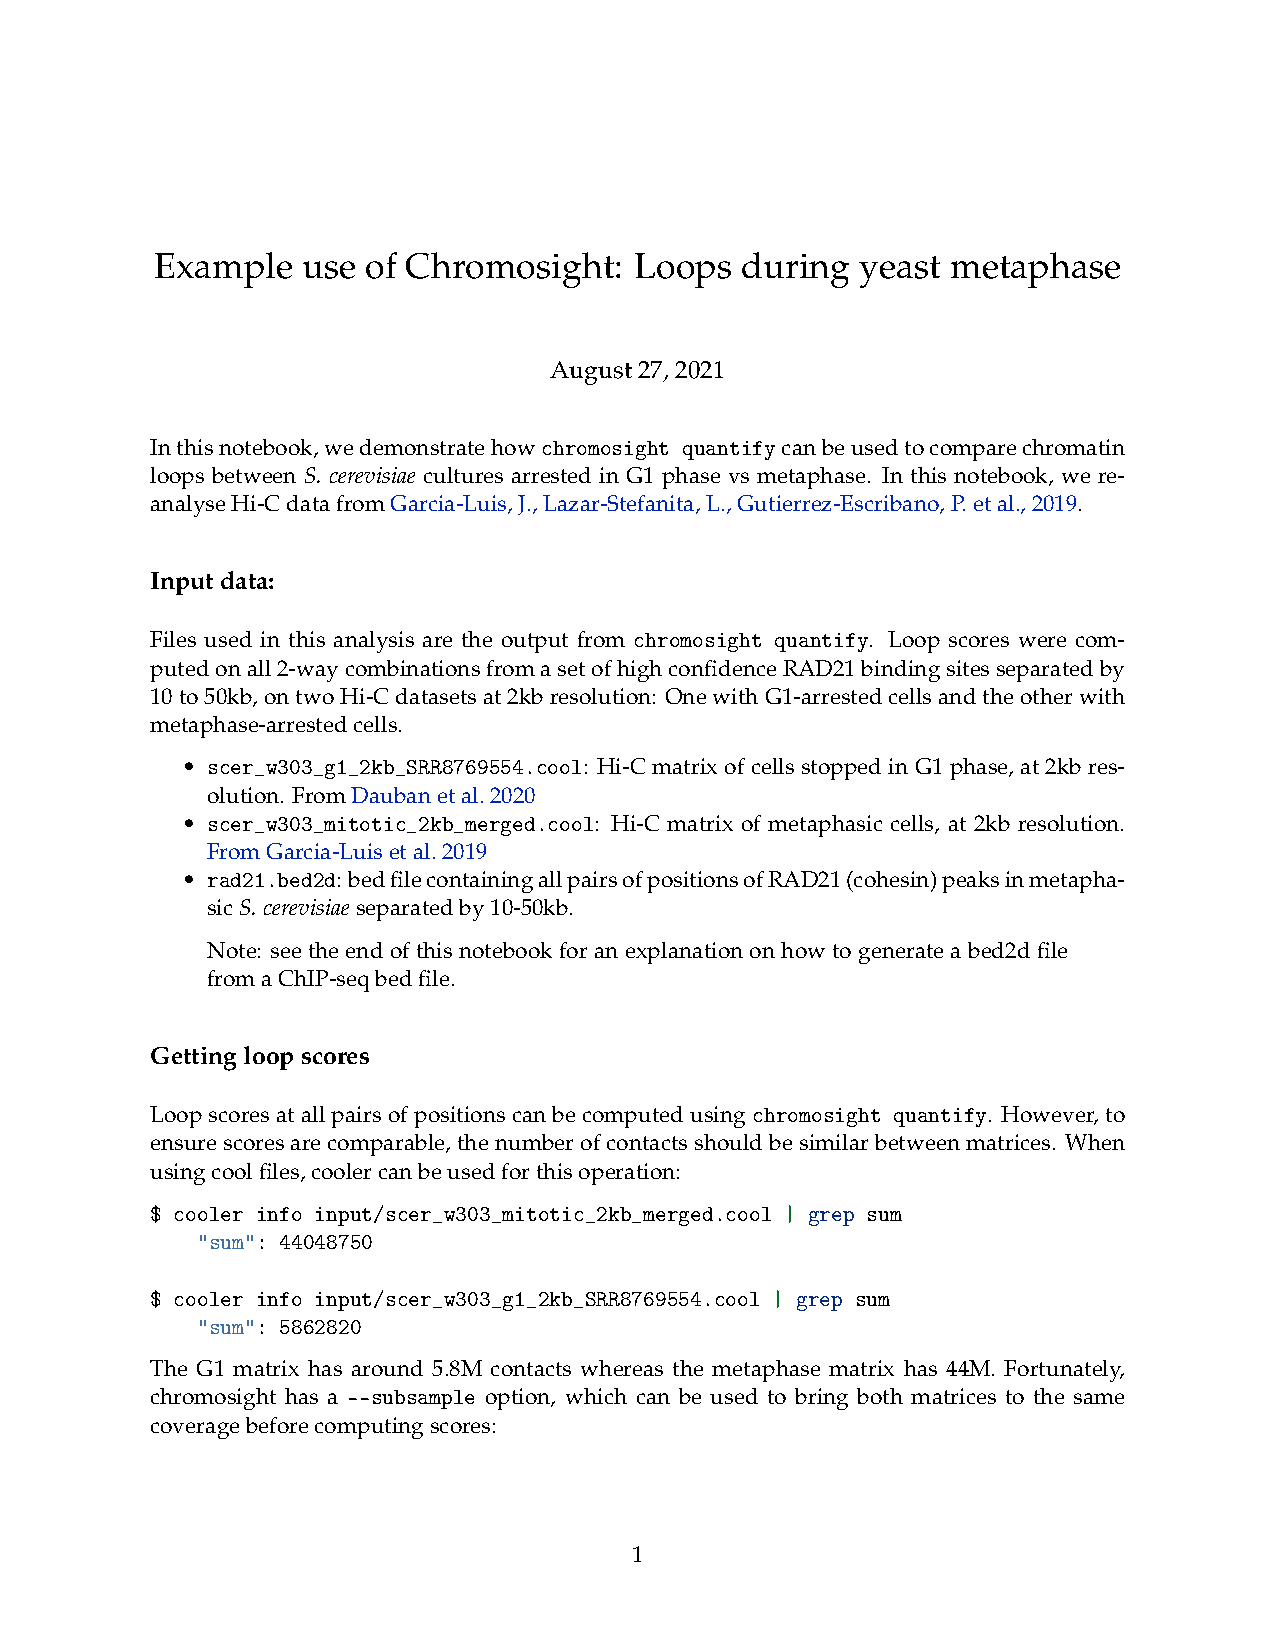
\includepdf[pages=-] {assets/g1_metaphase_yeast_example.pdf}    

\section{Output visualisation}
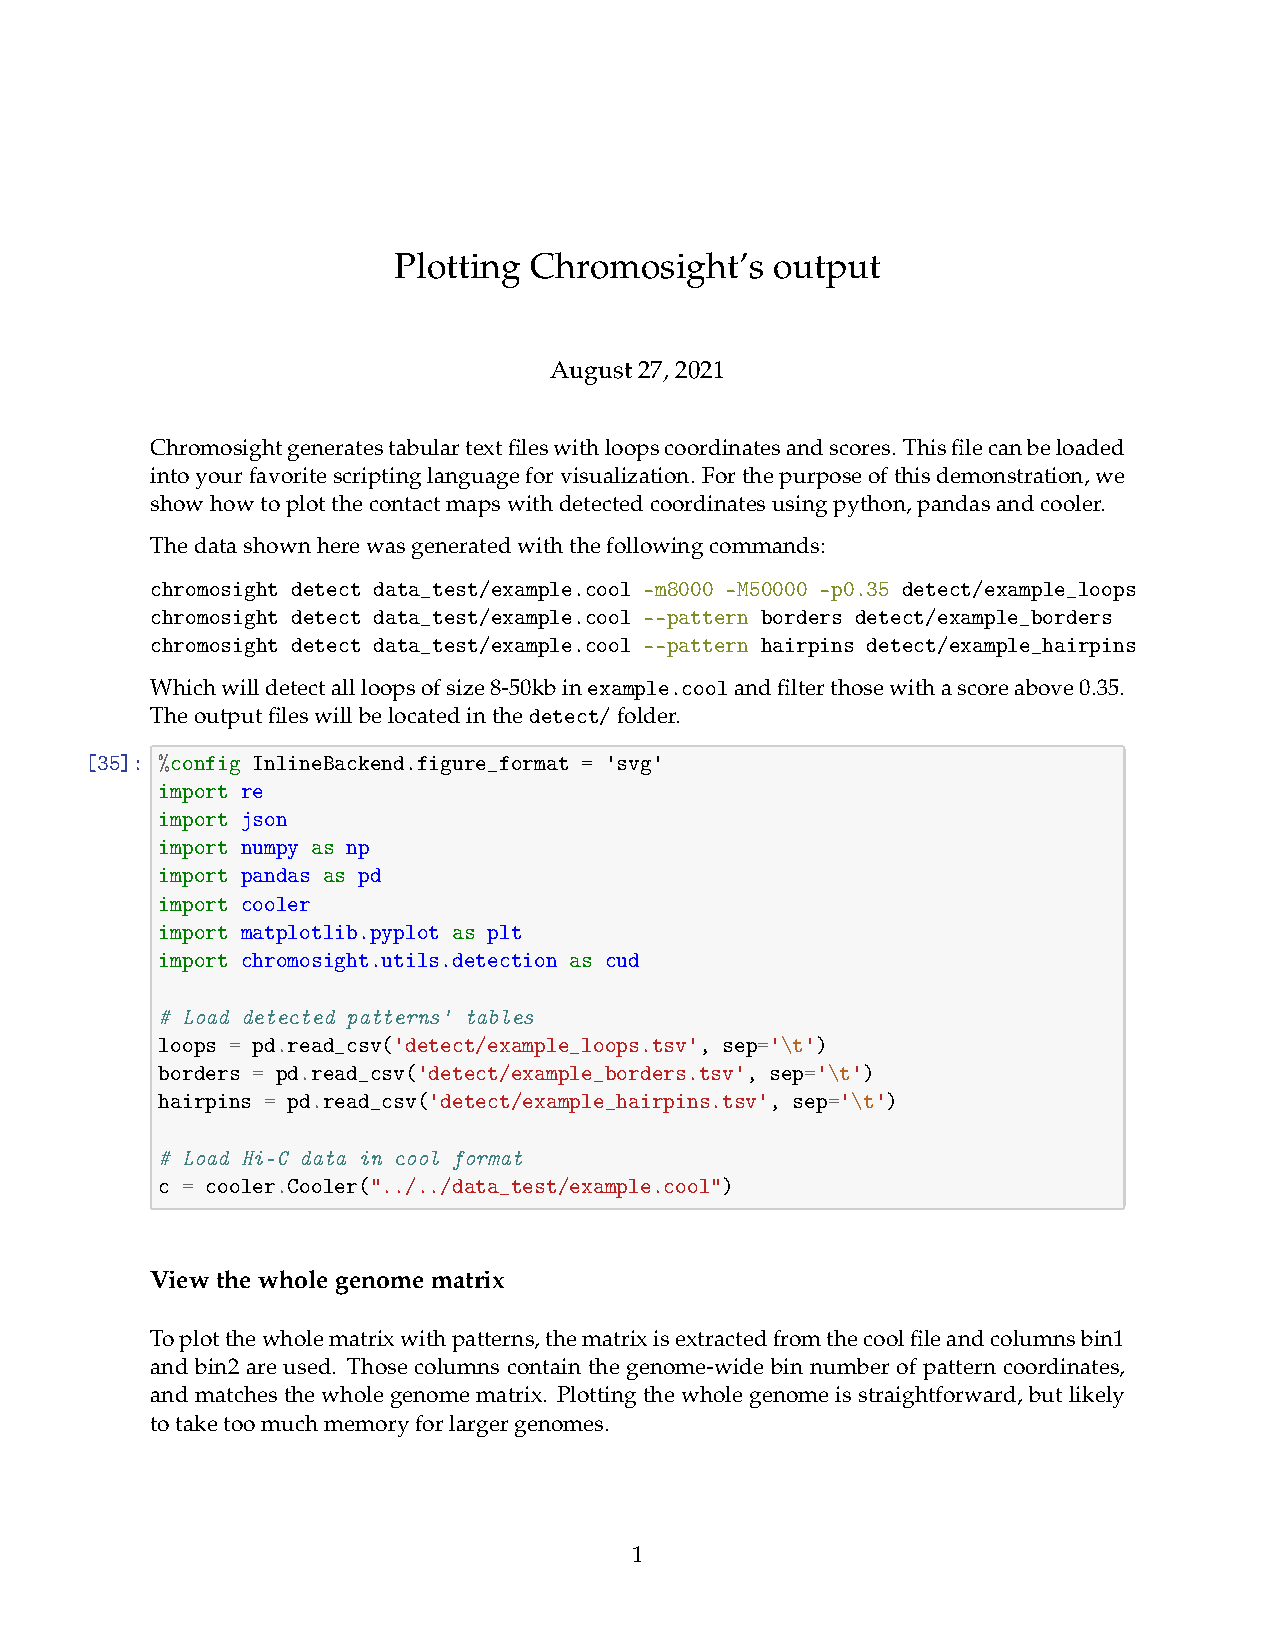
\includepdf[pages=-] {assets/plot_chromosight_output.pdf}

\chapter{Visual explanation of Pareidolia's algorithm}
\label{ch:04-C:pareidolia}

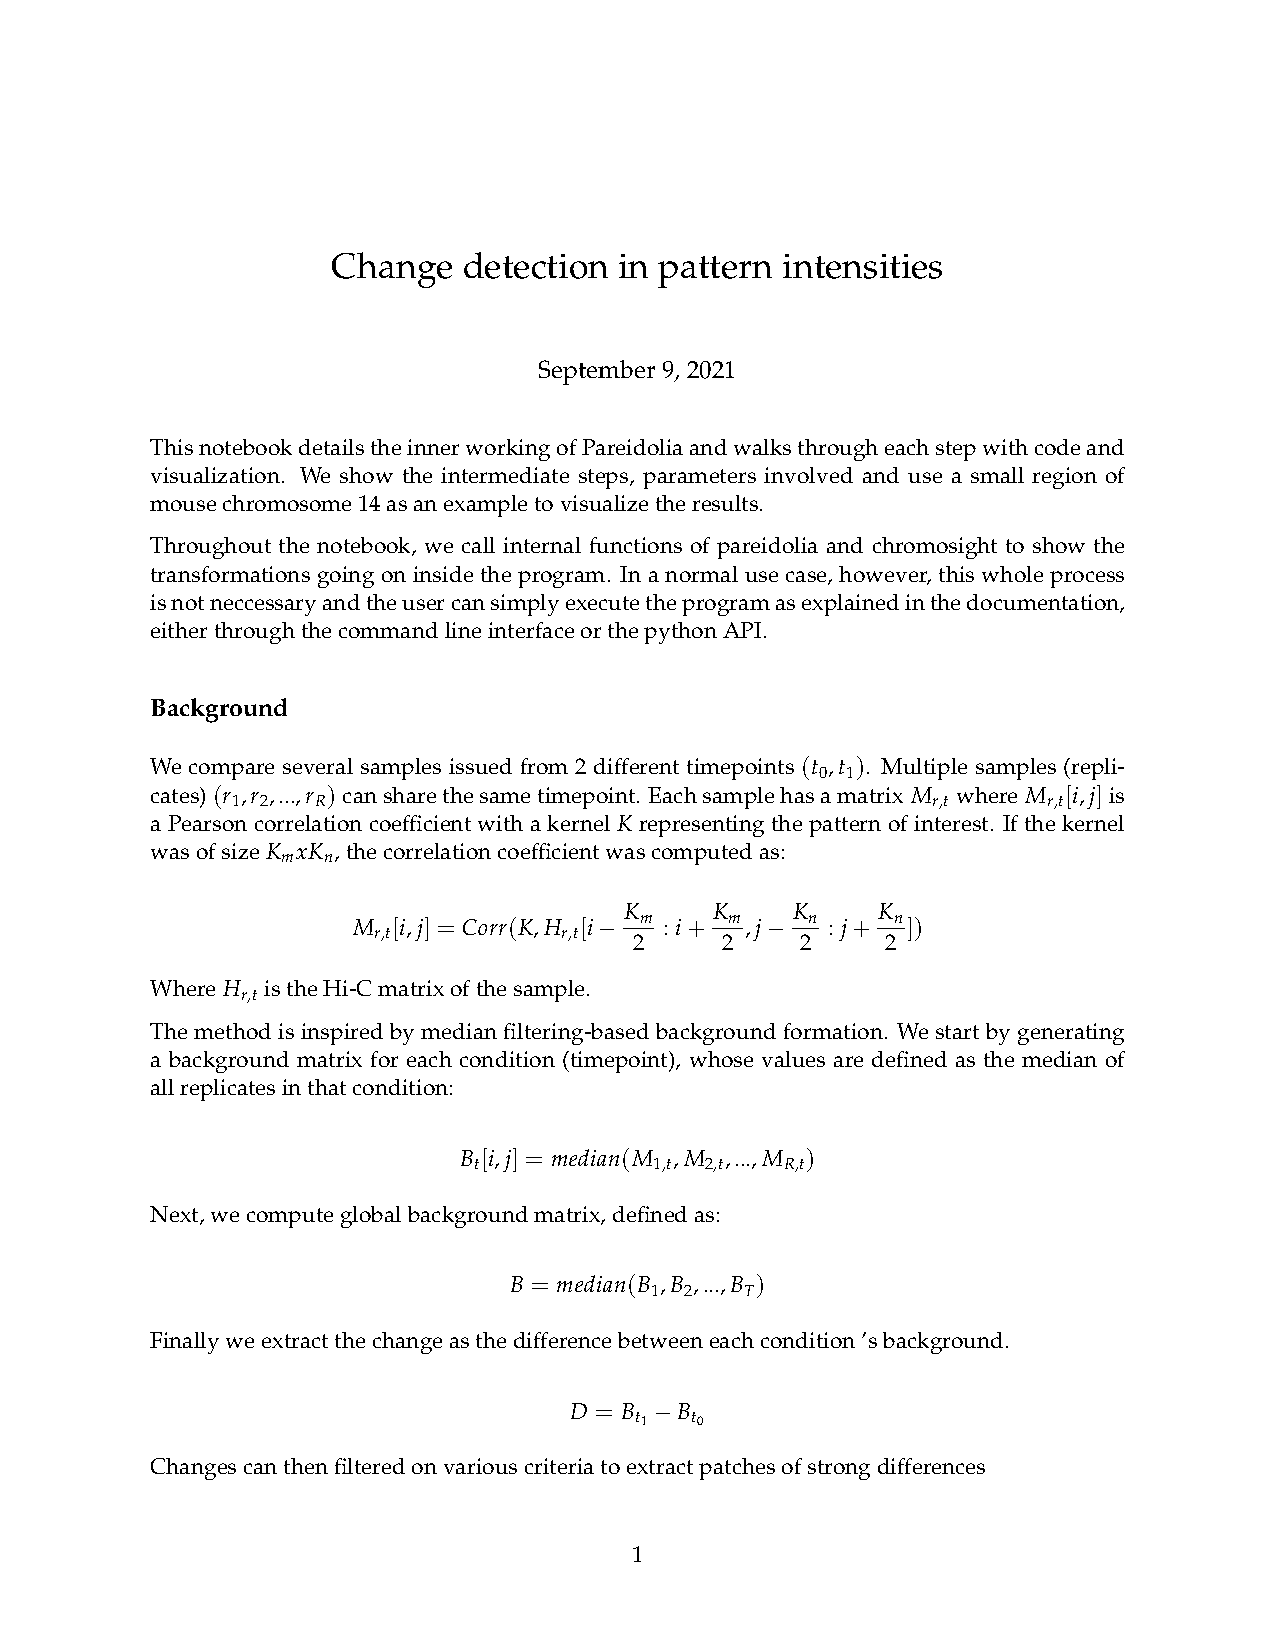
\includepdf[pages=-] {assets/pareidolia_change_detection.pdf}